% ============================================================
% Caption-Article Textual Similarity in News Media
% Compile with: pdflatex -> bibtex -> pdflatex -> pdflatex
% Overleaf: set compile root to paper/main.tex
% ============================================================
\documentclass[11pt,a4paper]{article}

% --- Encoding & fonts ---
\usepackage[T1]{fontenc}
\usepackage[utf8]{inputenc}
\usepackage{lmodern}
\usepackage{microtype}

% --- Page layout ---
\usepackage[margin=2.5cm]{geometry}

% --- Math & science ---
\usepackage{amsmath}
\usepackage{booktabs}
\usepackage{multirow}
\usepackage{array}

% --- Figures ---
\usepackage{graphicx}
\usepackage{subcaption}
\graphicspath{{../results/figures/}}   % figures generated by src/visualizations.py

% --- Tables from pandas to_latex() ---
% Each \input below pulls in a tabular environment only;
% wrap in table float for positioning.
\usepackage{adjustbox}

% --- Hyperlinks ---
\usepackage[colorlinks=true, linkcolor=blue, citecolor=blue, urlcolor=blue]{hyperref}

% --- Bibliography ---
\usepackage[numbers,sort&compress]{natbib}

% --- Misc ---
\usepackage{xcolor}
\usepackage{enumitem}
\setlength{\parskip}{4pt}

% ============================================================
\title{\textbf{Caption–Article Textual Similarity in News Media:\\
A Multi-Dimensional Analysis of the VisualNews Dataset}}

\author{
  Author One\thanks{Corresponding author.} \\
  School of Computer Science and Statistics \\
  Trinity College Dublin \\
  \texttt{author1@tcd.ie}
  \and
  Author Two \\
  School of Computer Science and Statistics \\
  Trinity College Dublin \\
  \texttt{author2@tcd.ie}
}

\date{}
% ============================================================

\begin{document}
\maketitle

% ============================================================
\begin{abstract}
Image captions in news articles perform a dual role: they anchor a photograph
to the surrounding text while simultaneously providing a concise, self-contained
narrative. How closely a caption tracks the lexical and semantic content of its
parent article, and what factors predict that alignment, remain open questions.
We present a systematic, multi-dimensional analysis of caption–article textual
similarity using 2,520 aligned pairs drawn from the VisualNews dataset, spanning
four major English-language news outlets and five topical categories.
We extract structural linguistic features from captions, compute three
complementary similarity metrics (TF-IDF cosine, lemma-set Jaccard, and SBERT
semantic similarity), perform named-entity alignment with fuzzy string matching,
and examine variation across news categories and publication sources.
Our findings indicate that \ldots\ [summarise key results here once full results
are available].
\end{abstract}

% ============================================================
\section{Introduction}
\label{sec:intro}

The relationship between a news photograph's caption and its accompanying
article text is fundamentally asymmetric: an article may run to hundreds of
words, while a caption rarely exceeds thirty \citep{alikhani-stone-2019-cite}.
Yet the two are expected to describe the same event.
Understanding \emph{how much} of the article's content a caption captures, and
through which linguistic mechanisms, has practical implications for automatic
caption generation, news summarisation, and multimodal fact-checking.

This paper addresses five research questions:

\begin{description}[leftmargin=2.5em, style=nextline]
  \item[RQ1] Do structural linguistic features of captions (length, syntactic
    complexity, vocabulary richness) predict caption–article similarity?
  \item[RQ2] Does the \emph{function} of a caption (e.g.\ descriptive,
    contextualising, evaluative) systematically vary in its degree of
    textual alignment with the article?
  \item[RQ3] Do named entities provide a reliable alignment signal, and
    does alignment differ by entity type?
  \item[RQ4] Does caption–article similarity vary across news topics
    (politics, sport, business, science, entertainment)?
  \item[RQ5] Are there cross-publication differences in caption–article
    alignment, and do UK outlets differ from US outlets?
\end{description}

We test five corresponding hypotheses (H1–H5, detailed in
Section~\ref{sec:method}) using both distributional statistics and
inferential tests on a 2,520-item stratified sample from VisualNews.

% ============================================================
\section{Related Work}
\label{sec:related}

\paragraph{Caption–image alignment.}
Early work on visual–linguistic grounding focused on image–sentence matching
\citep{Fang2015,Young2014}. More recently, large-scale datasets such as
VisualNews \citep{liu2020visualnews} and NewsCLIPpings \citep{luo2021newsclippings}
have enabled studies of caption veracity and cross-modal alignment.

\paragraph{Textual similarity in news.}
Lexical overlap metrics (BLEU, ROUGE) have been widely used for caption
evaluation \citep{Vedantam2015}. Embedding-based metrics such as BERTScore
\citep{zhang2020bertscore} and SBERT \citep{reimers-gurevych-2019-sentence}
offer complementary, semantics-sensitive assessments.

\paragraph{Named entity alignment.}
Entity-level overlap has been used as a factuality proxy in
summarisation \citep{Nan2021} and in cross-modal misinformation detection
\citep{Papadopoulos2023}. We extend this approach to caption–article pairs
with fuzzy matching to accommodate surface-form variation.

% ============================================================
\section{Data and Methodology}
\label{sec:method}

\subsection{Dataset}
We use VisualNews \citep{liu2020visualnews}, a large-scale dataset of
news images, captions, and full articles from four outlets: \emph{The Guardian},
\emph{BBC News}, \emph{USA Today}, and \emph{The Washington Post}.
After filtering to rows with non-empty article text, we retain 2,520 aligned
pairs. Table~\ref{tab:dataset} reports per-source statistics.

\begin{table}[h]
  \centering
  \caption{Dataset statistics per news source.}
  \label{tab:dataset}
  \adjustbox{max width=\linewidth}{%
    \begin{tabular}{lrlll}
\toprule
source & rows & avg caption words & avg article words & \% with entity overlap \\
\midrule
bbc & 822 & 13.2 & 413.7 & 59.4 \\
guardian & 1698 & 17.4 & 426.7 & 70.7 \\
\bottomrule
\end{tabular}
%
  }
\end{table}

\subsection{Preprocessing}
Text was Unicode-normalised (NFKC), stripped of HTML tags and entities, and
whitespace-standardised. Article text was truncated to the first 512
whitespace-delimited tokens to focus on the lead paragraph, which is most
likely to overlap with a caption.
Topic categories were consolidated from 30+ raw labels into five macro-categories:
\emph{politics\_government}, \emph{sport}, \emph{business\_economy},
\emph{science\_technology}, and \emph{entertainment\_culture}.

\subsection{Structural Feature Extraction}
All features are derived from captions using spaCy \texttt{en\_core\_web\_trf}.

\begin{itemize}[noitemsep]
  \item \textbf{Length}: token count, word count (alphabetic tokens), character
    count, sentence count.
  \item \textbf{Syntactic complexity}: average sentence length, maximum
    dependency tree depth, clause count (clausal dependency relations $+ 1$).
  \item \textbf{Vocabulary}: type–token ratio (TTR) over alphabetic lowercased
    tokens; content-word proportion (NOUN, VERB, ADJ, ADV); proper noun
    proportion.
  \item \textbf{POS overlap}: for each of NOUN, VERB, ADJ, PROPN, the
    fraction of caption lemmas of that type that also appear in the article:
    $|L^{cap}_{pos} \cap L^{art}_{pos}| \;/\; |L^{cap}_{pos}|$, or 0 if the
    caption set is empty.
\end{itemize}

\subsection{Similarity Metrics}

\paragraph{TF-IDF cosine ($s_{tf}$).}
A \texttt{TfidfVectorizer} (bigrams, $\text{min\_df}=2$, $\text{max\_df}=0.95$)
is fit on the combined caption+article corpus; per-pair cosine similarity is
computed between the caption and article vectors.

\paragraph{Jaccard similarity ($s_{jac}$).}
Both texts are lemmatised with spaCy; stopwords and punctuation are removed;
Jaccard similarity is computed over the resulting lemma sets:
$|C \cap A| \;/\; |C \cup A|$.

\paragraph{SBERT similarity ($s_{sbert}$).}
Caption and article embeddings are produced by
\texttt{all-MiniLM-L6-v2} \citep{reimers-gurevych-2019-sentence} with
\texttt{batch\_size=64}; cosine similarity is computed over $\ell_2$-normalised
vectors.

\subsection{Named-Entity Alignment}
Entities of type PERSON, GPE, ORG, and DATE are extracted with
\texttt{en\_core\_web\_trf}. Two entity strings are considered a match if their
Levenshtein similarity $\geq 0.85$ (computed via \texttt{rapidfuzz}).
Per entity type we report \emph{overlap rate}
$= |E^{cap} \cap E^{art}| / |E^{cap}|$;
globally we report \emph{entity Jaccard}
$= |E^{cap} \cap E^{art}| / |E^{cap} \cup E^{art}|$
and \emph{coverage rate} $= |E^{cap} \cap E^{art}| / |E^{art}|$.

\subsection{Statistical Analysis}
Pearson $r$ (two-tailed) is used for correlation tests.
Group comparisons use the Kruskal–Wallis $H$ test followed by
Dunn's post-hoc test with Bonferroni correction for pairwise source
comparisons. Effect size is reported as
$\eta^2 = (H - k + 1) / (n - k)$.
Significance threshold: $\alpha = 0.05$.

\subsection{Hypotheses}
\begin{description}[leftmargin=2.5em, style=nextline]
  \item[H1] At least one structural feature (esp.\ word count or TTR)
    significantly correlates with caption–article similarity.
  \item[H2] Caption function (type) significantly predicts similarity across
    all three metrics.
  \item[H3] Entity overlap rates differ by type; PERSON overlap is highest
    given its specificity.
  \item[H4] Caption–article similarity varies significantly across news
    categories, with sport showing higher alignment due to precise event
    descriptions.
  \item[H5] UK outlets (Guardian, BBC) exhibit higher caption–article
    similarity than US outlets (WaPo, USA Today).
\end{description}

% ============================================================
\section{Results}
\label{sec:results}

\subsection{Descriptive Overview}

Figure~\ref{fig:cap_len} shows the caption word-count distribution, which is
right-skewed with a median of approximately 20 words. The distributions of the
three similarity scores (Figure~\ref{fig:sim_dist}) reveal that $s_{sbert}$
occupies a higher range than $s_{tf}$ and $s_{jac}$, reflecting its sensitivity
to paraphrase rather than surface overlap.

\begin{figure}[h]
  \centering
  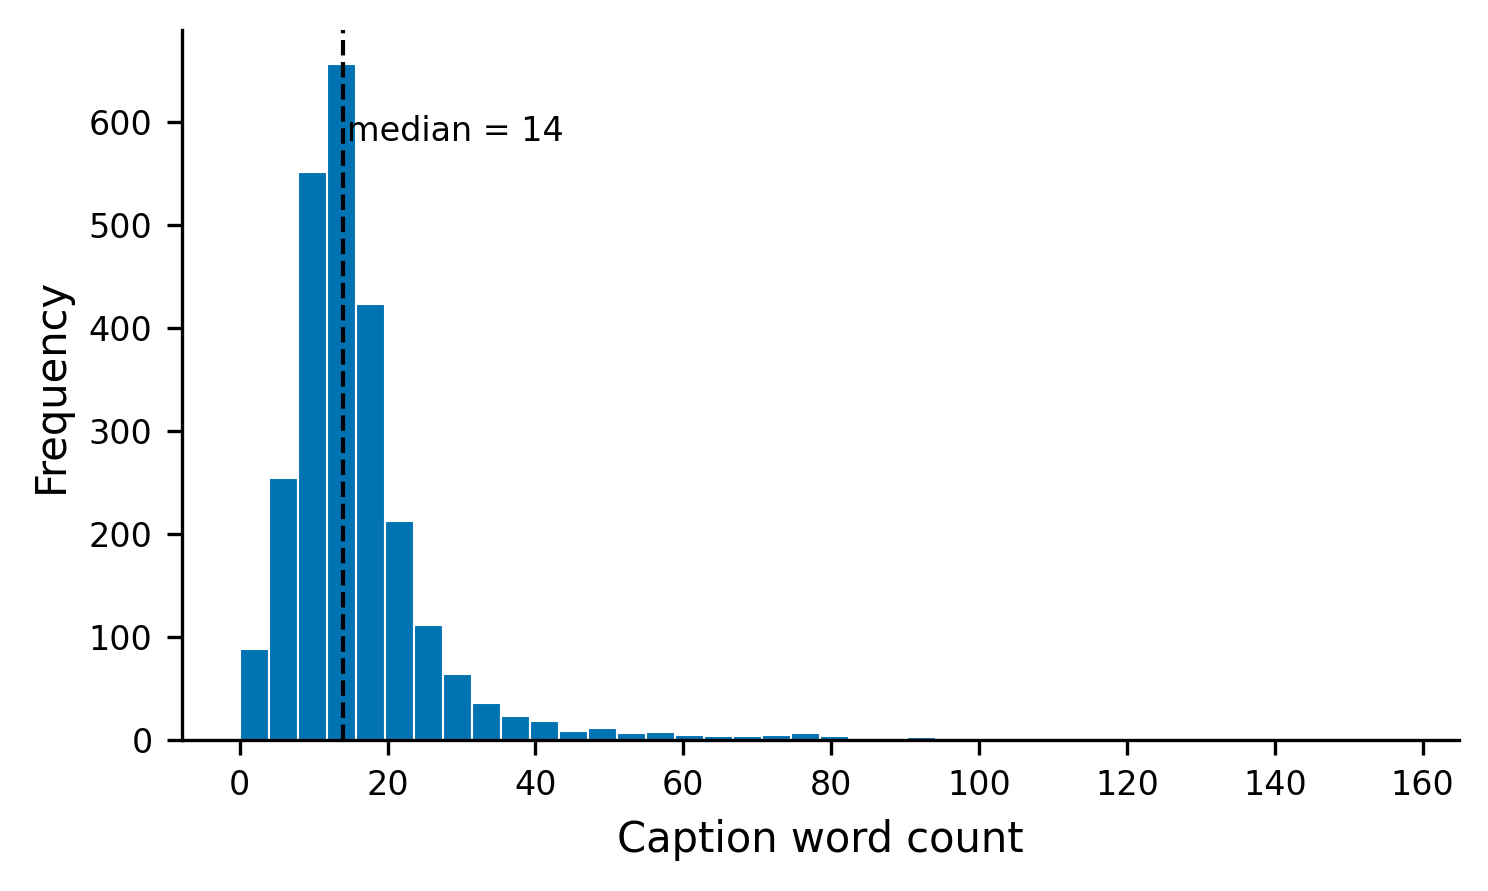
\includegraphics[width=0.85\linewidth]{caption_length_distribution.png}
  \caption{Distribution of caption word counts (median annotated).}
  \label{fig:cap_len}
\end{figure}

\begin{figure}[h]
  \centering
  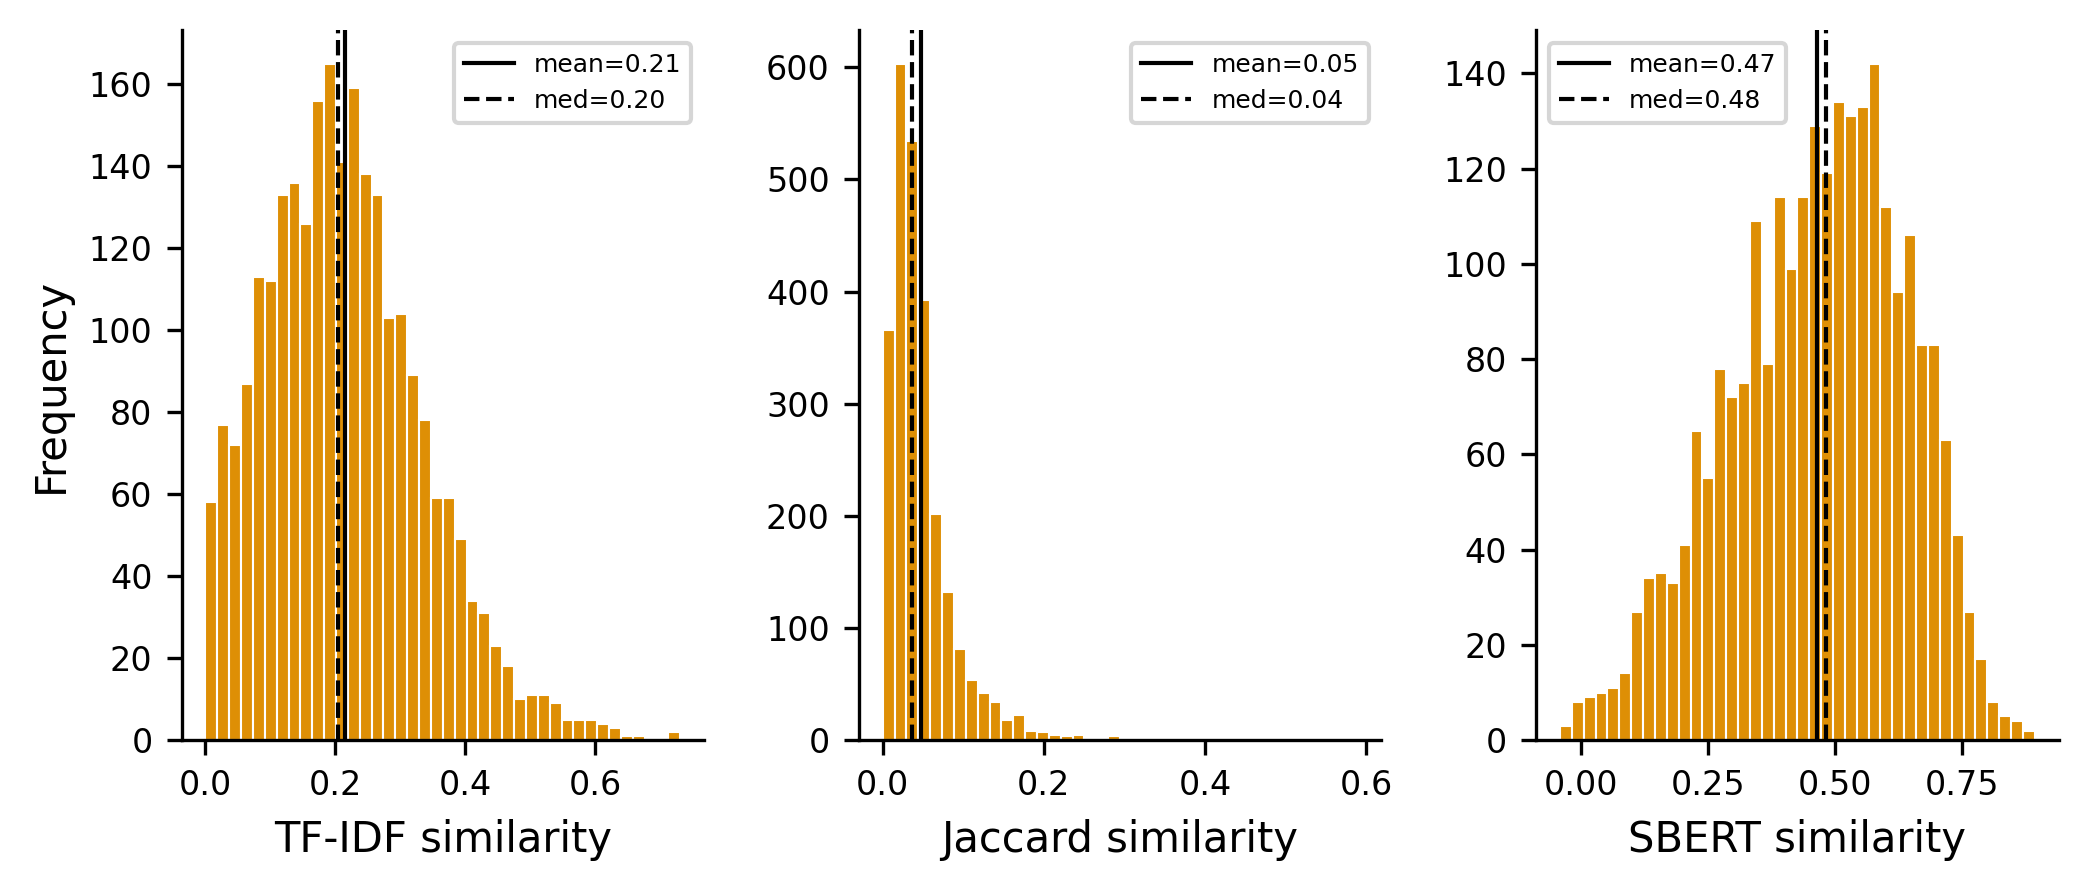
\includegraphics[width=\linewidth]{similarity_score_distributions.png}
  \caption{Distributions of TF-IDF cosine, Jaccard, and SBERT similarity scores.
           Mean (solid) and median (dashed) are annotated.}
  \label{fig:sim_dist}
\end{figure}

% -------------------------------------------------------
\subsection{RQ1: Structural Features and Similarity}
\label{sec:rq1}

Figure~\ref{fig:rq1_heat} presents the Pearson correlation matrix between
structural caption features and the three similarity measures. Cells marked
with~* indicate $p < 0.05$.

\begin{figure}[h]
  \centering
  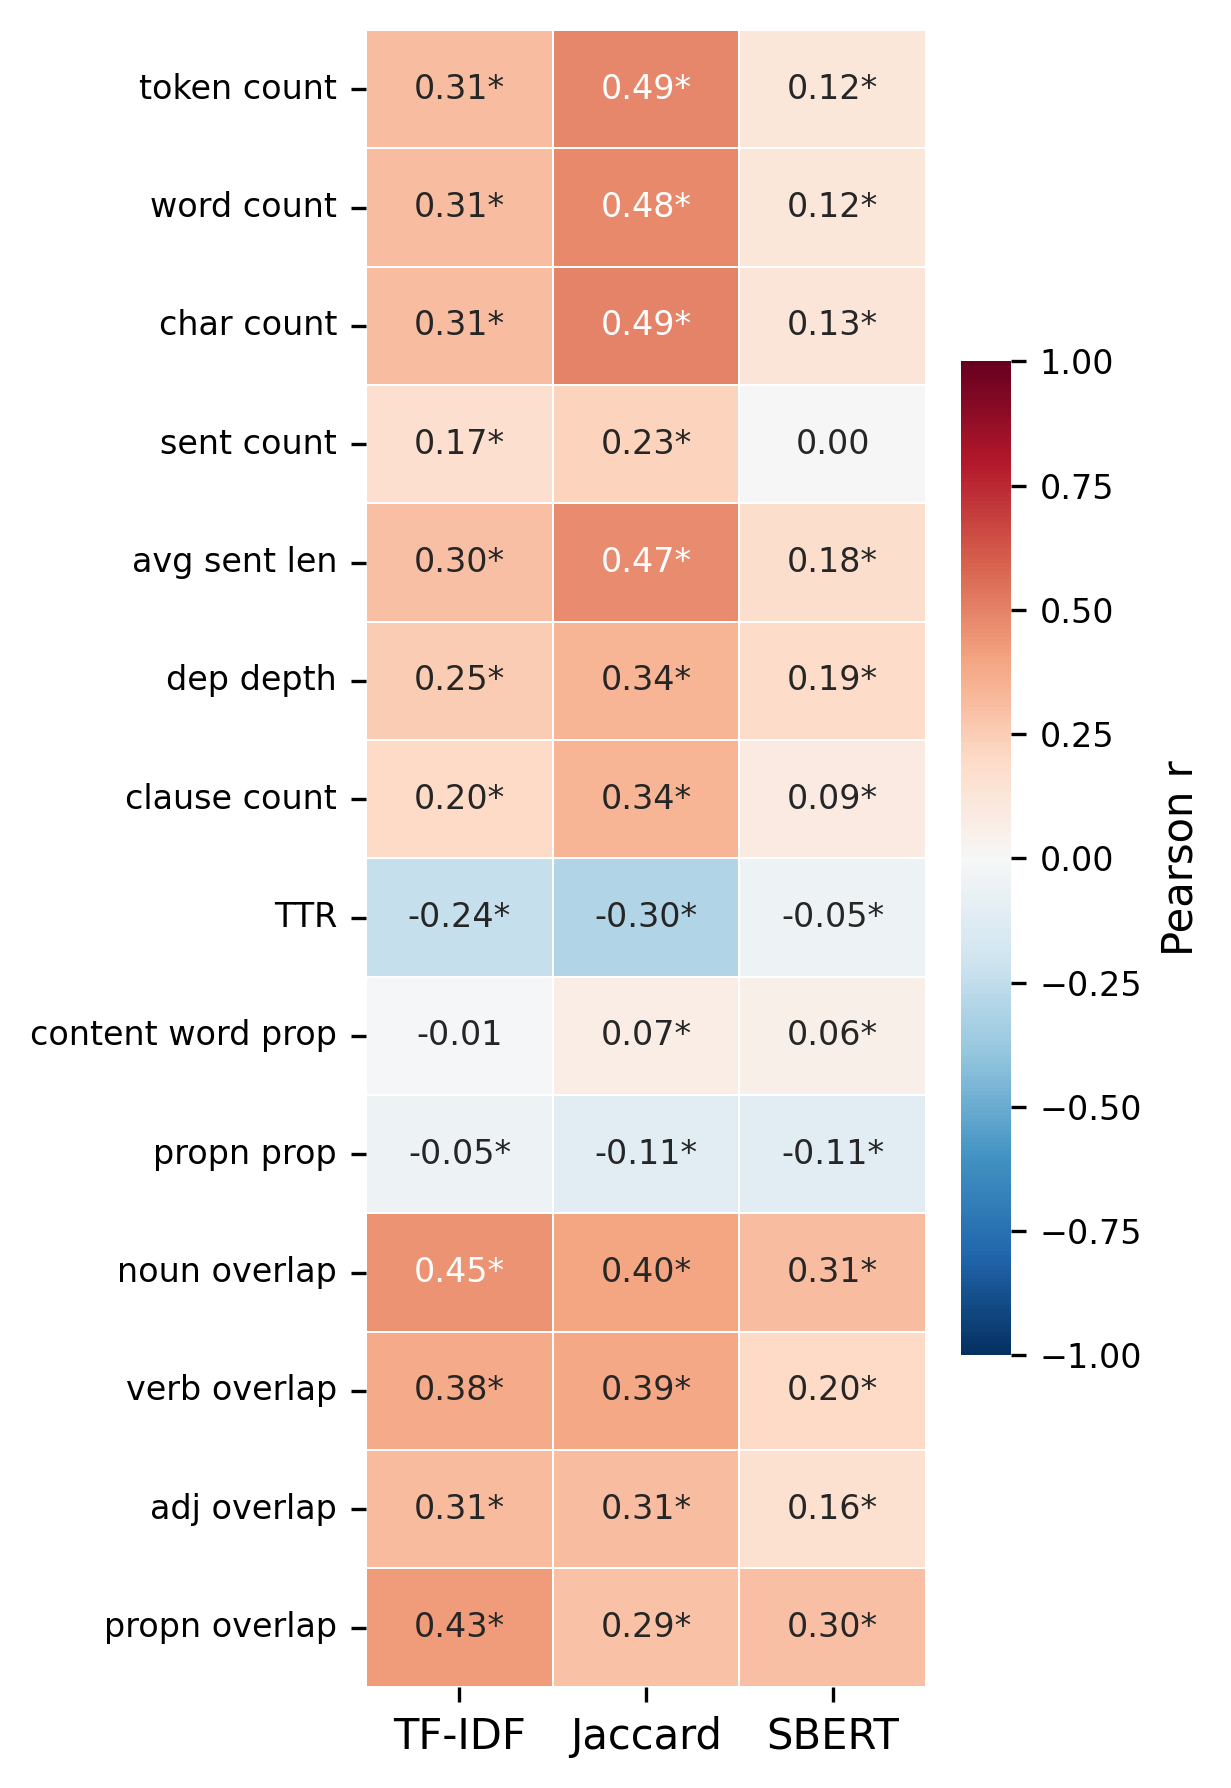
\includegraphics[width=0.7\linewidth]{rq1_correlation_heatmap.png}
  \caption{Pearson $r$ between structural features and similarity measures.
           * denotes $p < 0.05$.}
  \label{fig:rq1_heat}
\end{figure}

Figure~\ref{fig:rq1_scatter} shows scatter plots for the three strongest
significant correlations with regression lines (95\% CI).

\begin{figure}[h]
  \centering
  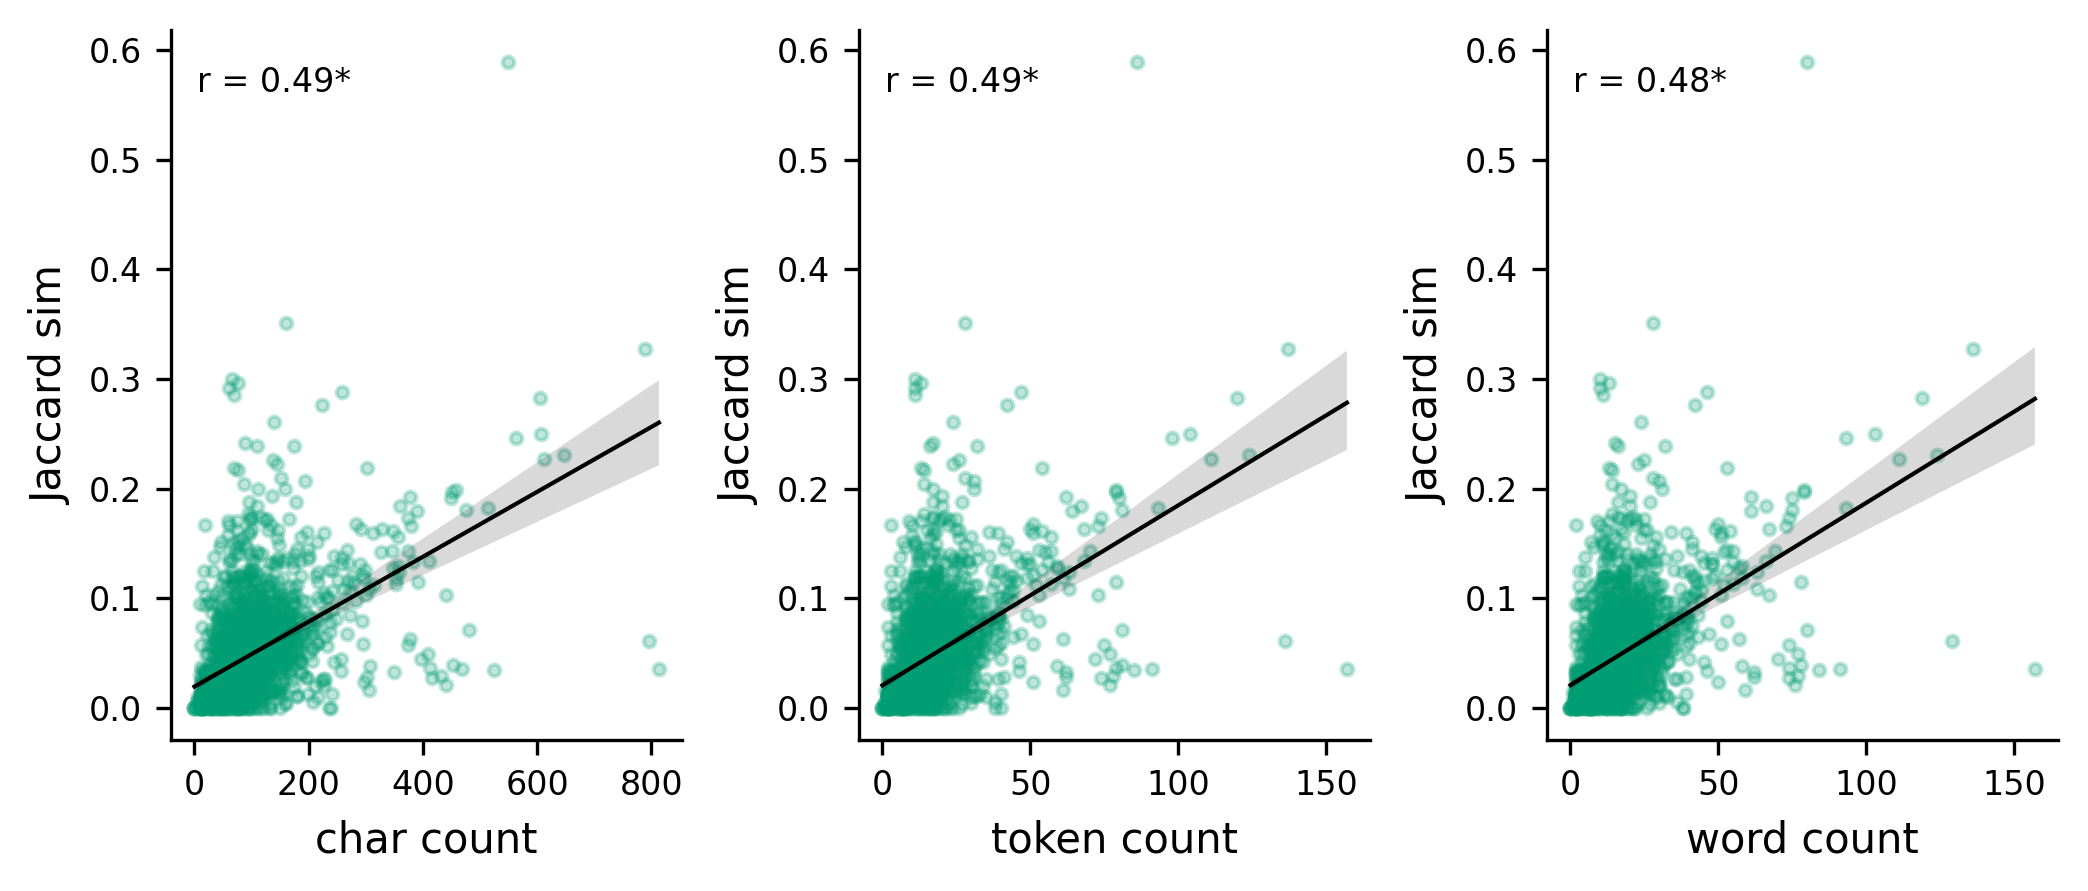
\includegraphics[width=\linewidth]{rq1_top_scatter.png}
  \caption{Top three significant structural feature–similarity correlations.}
  \label{fig:rq1_scatter}
\end{figure}

The full correlation table with $r$ and $p$-values is reported in
Table~\ref{tab:rq1}. [Interpret key findings here.]

\begin{table}[h]
  \centering
  \caption{Pearson $r$ and $p$-values for structural features vs.\ similarity
           measures. * $p < 0.05$.}
  \label{tab:rq1}
  \adjustbox{max width=\linewidth}{%
    \begin{tabular}{lllllll}
\toprule
feature & r (TF-IDF) & p (TF-IDF) & r (Jaccard) & p (Jaccard) & r (SBERT) & p (SBERT) \\
\midrule
noun overlap & 0.453 & 0.000* & 0.398 & 0.000* & 0.306 & 0.000* \\
propn overlap & 0.426 & 0.000* & 0.291 & 0.000* & 0.304 & 0.000* \\
verb overlap & 0.377 & 0.000* & 0.387 & 0.000* & 0.197 & 0.000* \\
dep depth & 0.252 & 0.000* & 0.343 & 0.000* & 0.189 & 0.000* \\
avg sent len & 0.302 & 0.000* & 0.469 & 0.000* & 0.179 & 0.000* \\
adj overlap & 0.314 & 0.000* & 0.305 & 0.000* & 0.163 & 0.000* \\
char count & 0.312 & 0.000* & 0.494 & 0.000* & 0.132 & 0.000* \\
token count & 0.312 & 0.000* & 0.487 & 0.000* & 0.121 & 0.000* \\
word count & 0.308 & 0.000* & 0.484 & 0.000* & 0.120 & 0.000* \\
propn prop & -0.048 & 0.016* & -0.111 & 0.000* & -0.110 & 0.000* \\
clause count & 0.200 & 0.000* & 0.342 & 0.000* & 0.094 & 0.000* \\
content word prop & -0.008 & 0.690 & 0.074 & 0.000* & 0.059 & 0.003* \\
TTR & -0.239 & 0.000* & -0.301 & 0.000* & -0.052 & 0.009* \\
sent count & 0.169 & 0.000* & 0.234 & 0.000* & 0.000 & 0.995 \\
\bottomrule
\end{tabular}
%
  }
\end{table}

% -------------------------------------------------------
\subsection{RQ2: Caption Function and Similarity}
\label{sec:rq2}

% NOTE: Uncomment once caption_classifier.py is implemented.
% Figure~\ref{fig:rq2} shows similarity distributions per caption type.
%
% \begin{figure}[h]
%   \centering
%   \includegraphics[width=\linewidth]{rq2_similarity_by_type.png}
%   \caption{Similarity distributions by caption type (box + strip).}
%   \label{fig:rq2}
% \end{figure}
%
% \begin{table}[h]
%   \centering
%   \caption{Mean $\pm$ SD similarity by caption type; Kruskal-Wallis result.}
%   \label{tab:rq2}
%   \adjustbox{max width=\linewidth}{%
%     \input{../results/figures/table_rq2_similarity_by_type}%
%   }
% \end{table}

\noindent\textit{RQ2 figures will be populated once caption type classification
is finalised (see \texttt{src/caption\_classifier.py}).}

% -------------------------------------------------------
\subsection{RQ3: Named-Entity Alignment}
\label{sec:rq3}

Figure~\ref{fig:rq3_bar} shows mean entity overlap rate per entity type with
95\% confidence intervals. Figure~\ref{fig:rq3_scatter} plots entity Jaccard
against SBERT similarity, coloured by source.

\begin{figure}[h]
  \centering
  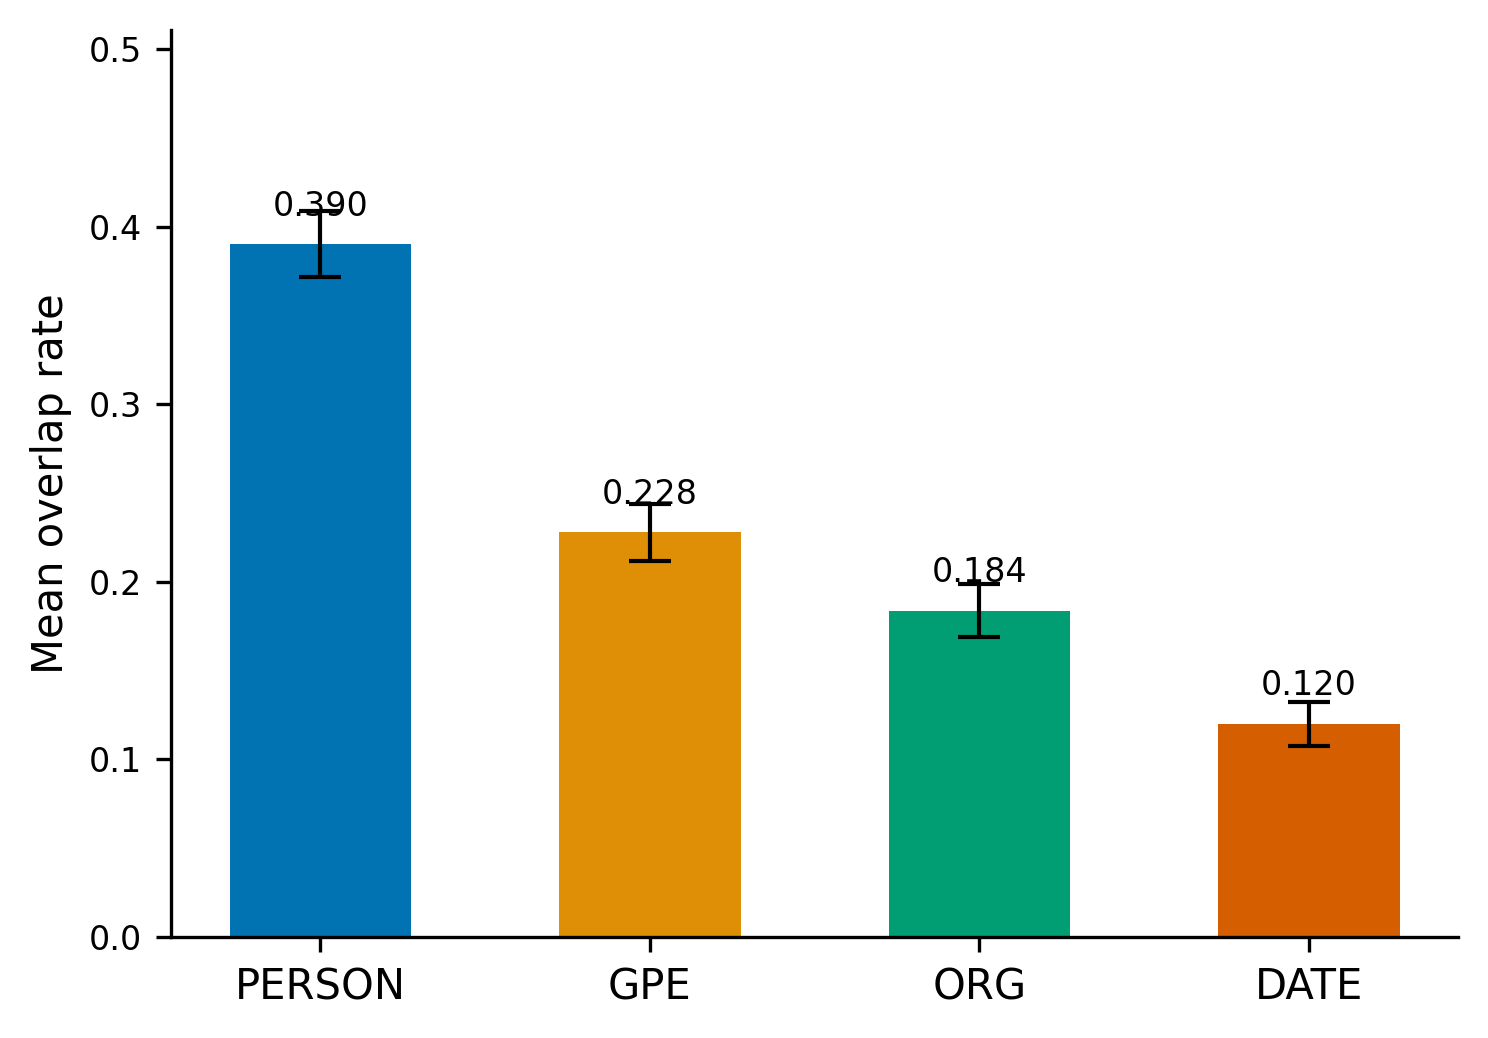
\includegraphics[width=0.85\linewidth]{rq3_entity_overlap_by_type.png}
  \caption{Mean entity overlap rate per type (error bars: 95\% CI).}
  \label{fig:rq3_bar}
\end{figure}

\begin{figure}[h]
  \centering
  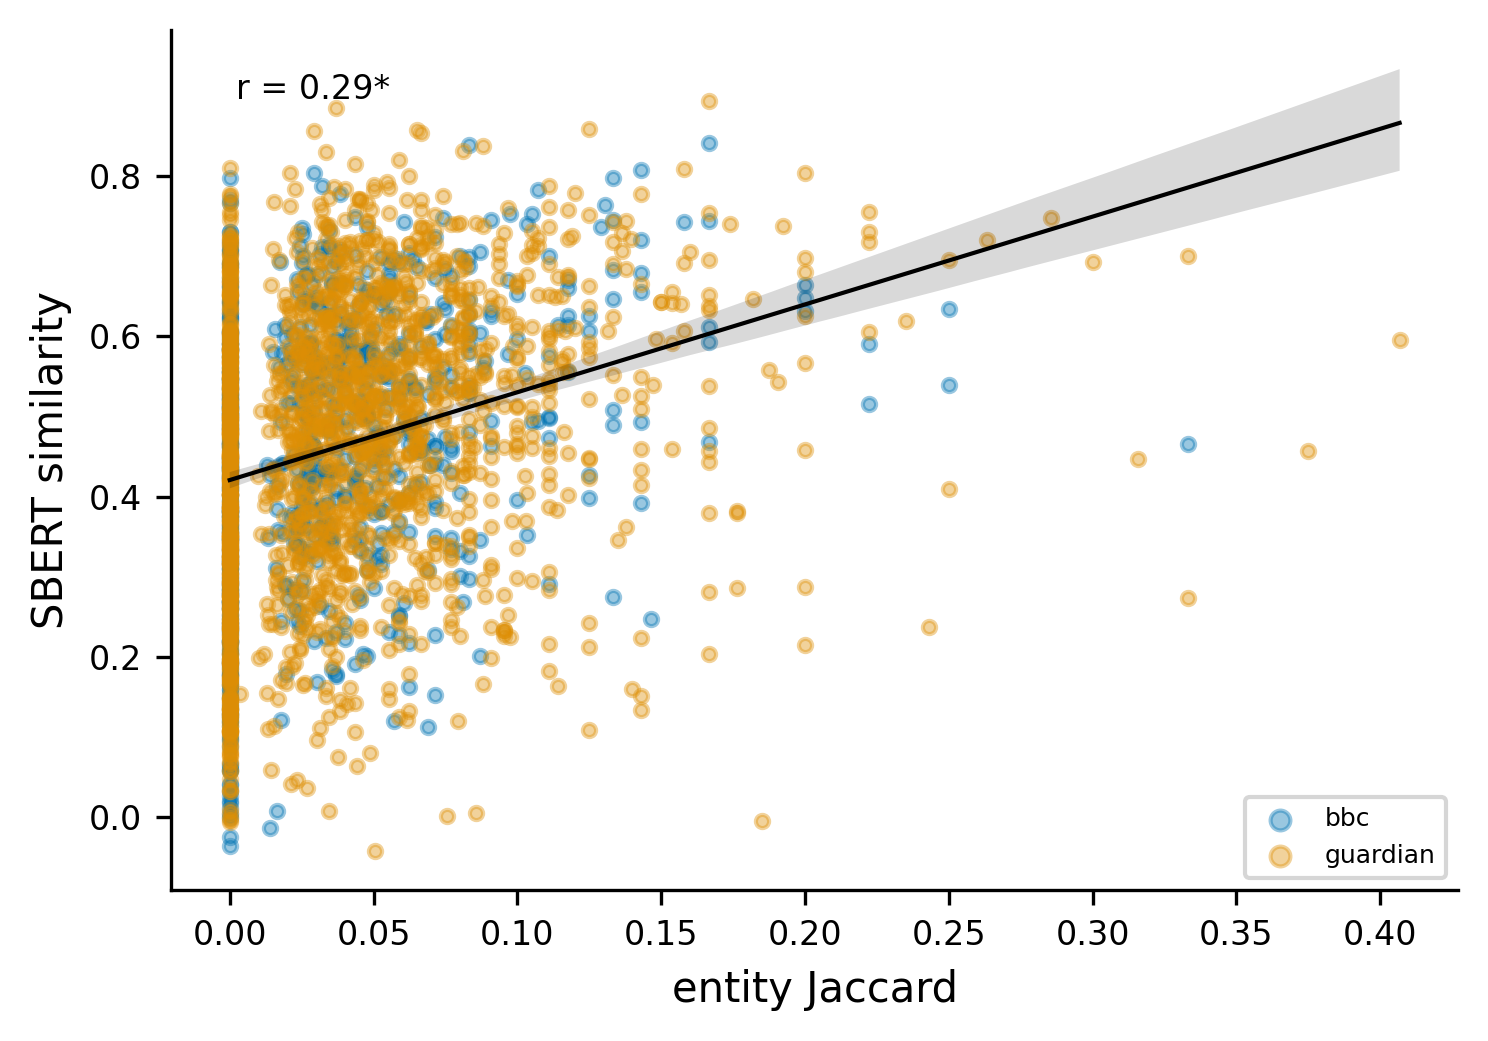
\includegraphics[width=0.85\linewidth]{rq3_entity_jaccard_vs_sbert.png}
  \caption{Entity Jaccard vs.\ SBERT similarity, coloured by source.}
  \label{fig:rq3_scatter}
\end{figure}

\begin{table}[h]
  \centering
  \caption{Mean entity alignment metrics per entity type.
           Coverage rate and Jaccard are reported for the overall row only
           (per-type coverage not available from the pipeline output).}
  \label{tab:rq3}
  \adjustbox{max width=\linewidth}{%
    \begin{tabular}{llll}
\toprule
entity type & mean overlap & mean coverage & mean jaccard \\
\midrule
PERSON & 0.390 & — & — \\
GPE & 0.228 & — & — \\
ORG & 0.184 & — & — \\
DATE & 0.120 & — & — \\
Overall & 0.230 & 0.041 & 0.041 \\
\bottomrule
\end{tabular}
%
  }
\end{table}

% -------------------------------------------------------
\subsection{RQ4: News Category}
\label{sec:rq4}

\begin{figure}[h]
  \centering
  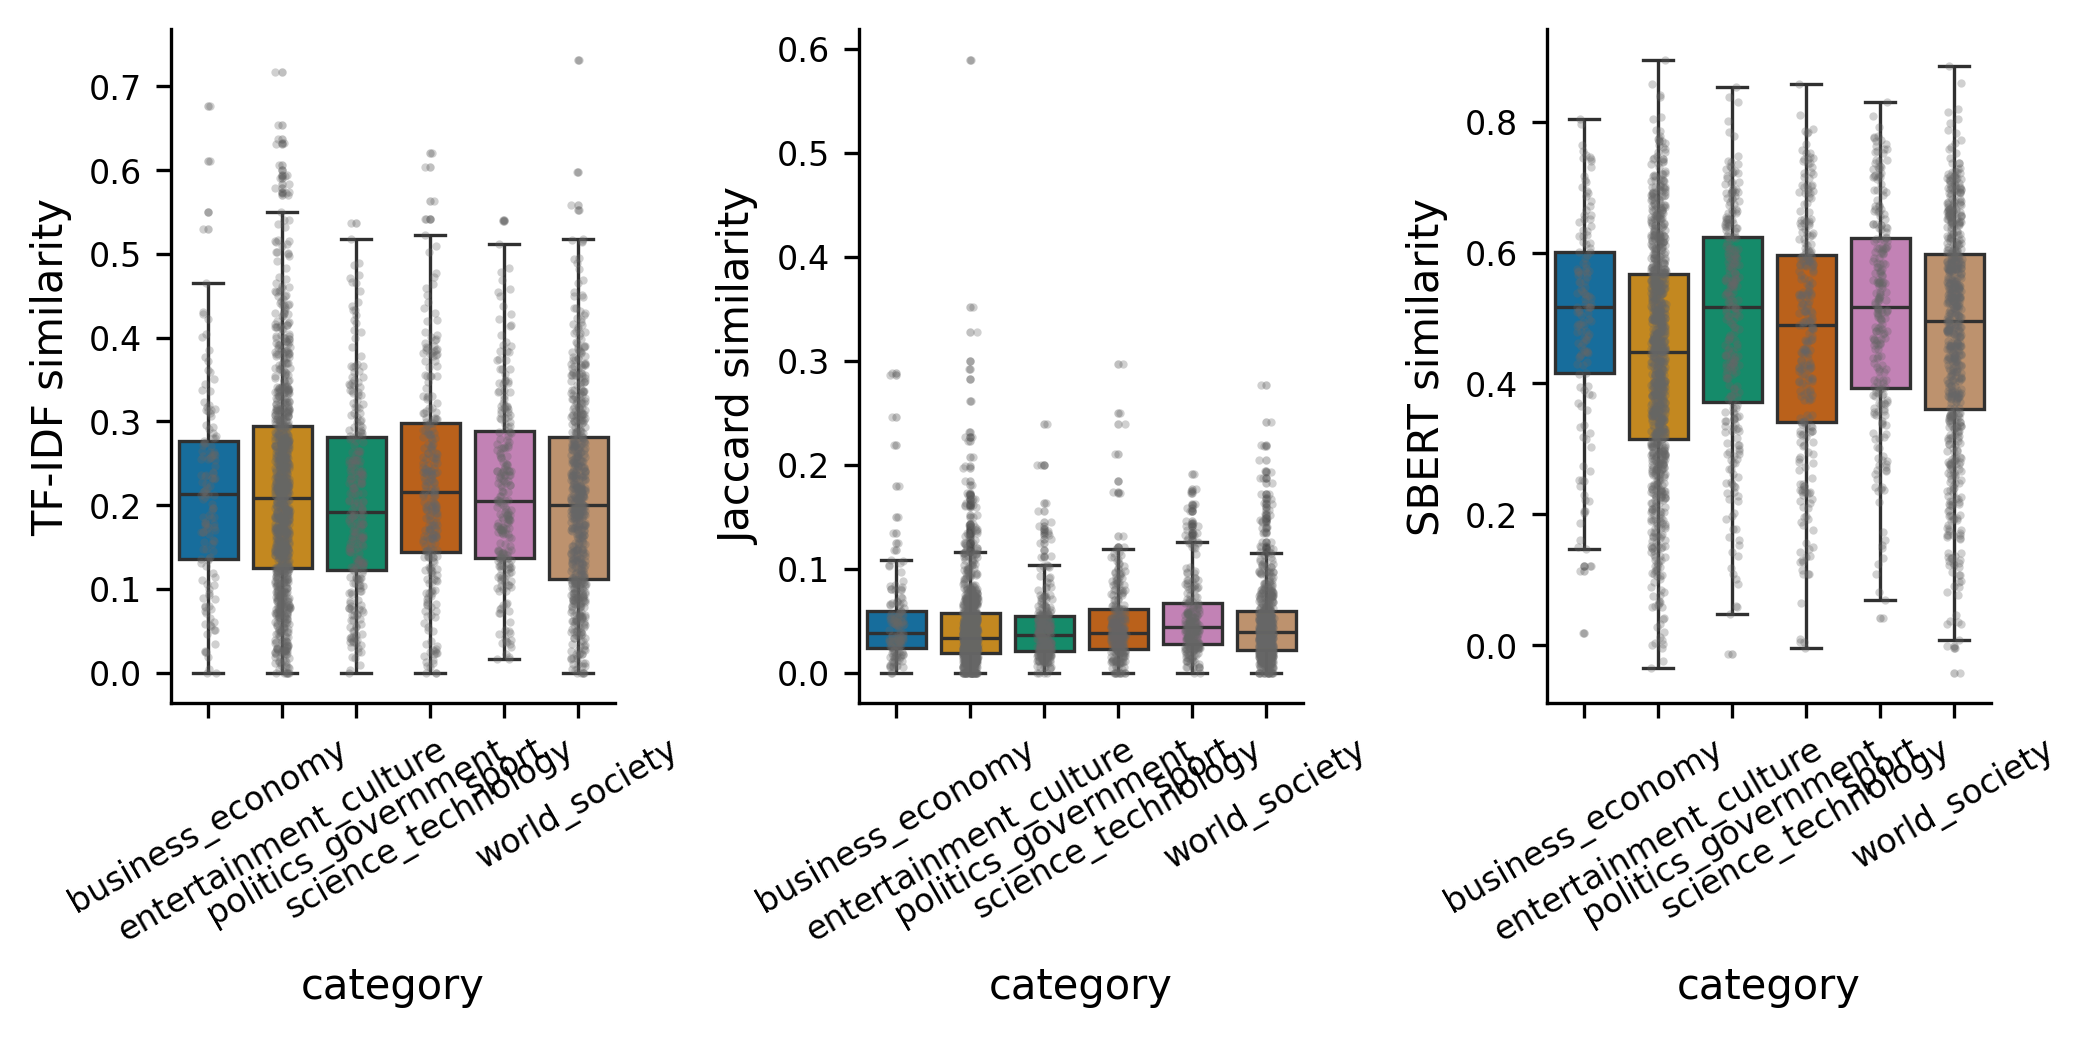
\includegraphics[width=\linewidth]{rq4_similarity_by_category.png}
  \caption{Similarity distributions by news category.}
  \label{fig:rq4}
\end{figure}

\begin{table}[h]
  \centering
  \caption{Mean $\pm$ SD similarity by news category; Kruskal-Wallis result.}
  \label{tab:rq4}
  \adjustbox{max width=\linewidth}{%
    \begin{tabular}{llll}
\toprule
category & TF-IDF & Jaccard & SBERT \\
\midrule
business\_economy & 0.215 ± 0.121 & 0.051 ± 0.048 & 0.493 ± 0.164 \\
entertainment\_culture & 0.218 ± 0.126 & 0.046 ± 0.046 & 0.437 ± 0.172 \\
politics\_government & 0.205 ± 0.115 & 0.044 ± 0.035 & 0.491 ± 0.171 \\
science\_technology & 0.225 ± 0.122 & 0.048 ± 0.040 & 0.469 ± 0.181 \\
sport & 0.218 ± 0.109 & 0.054 ± 0.039 & 0.507 ± 0.164 \\
world\_society & 0.207 ± 0.116 & 0.047 ± 0.039 & 0.474 ± 0.171 \\
Kruskal-Wallis & H=6.16, p=0.291 & H=24.52, p=0.000 & H=54.08, p=0.000 \\
\bottomrule
\end{tabular}
%
  }
\end{table}

% -------------------------------------------------------
\subsection{RQ5: Cross-Source Analysis}
\label{sec:rq5}

\begin{figure}[h]
  \centering
  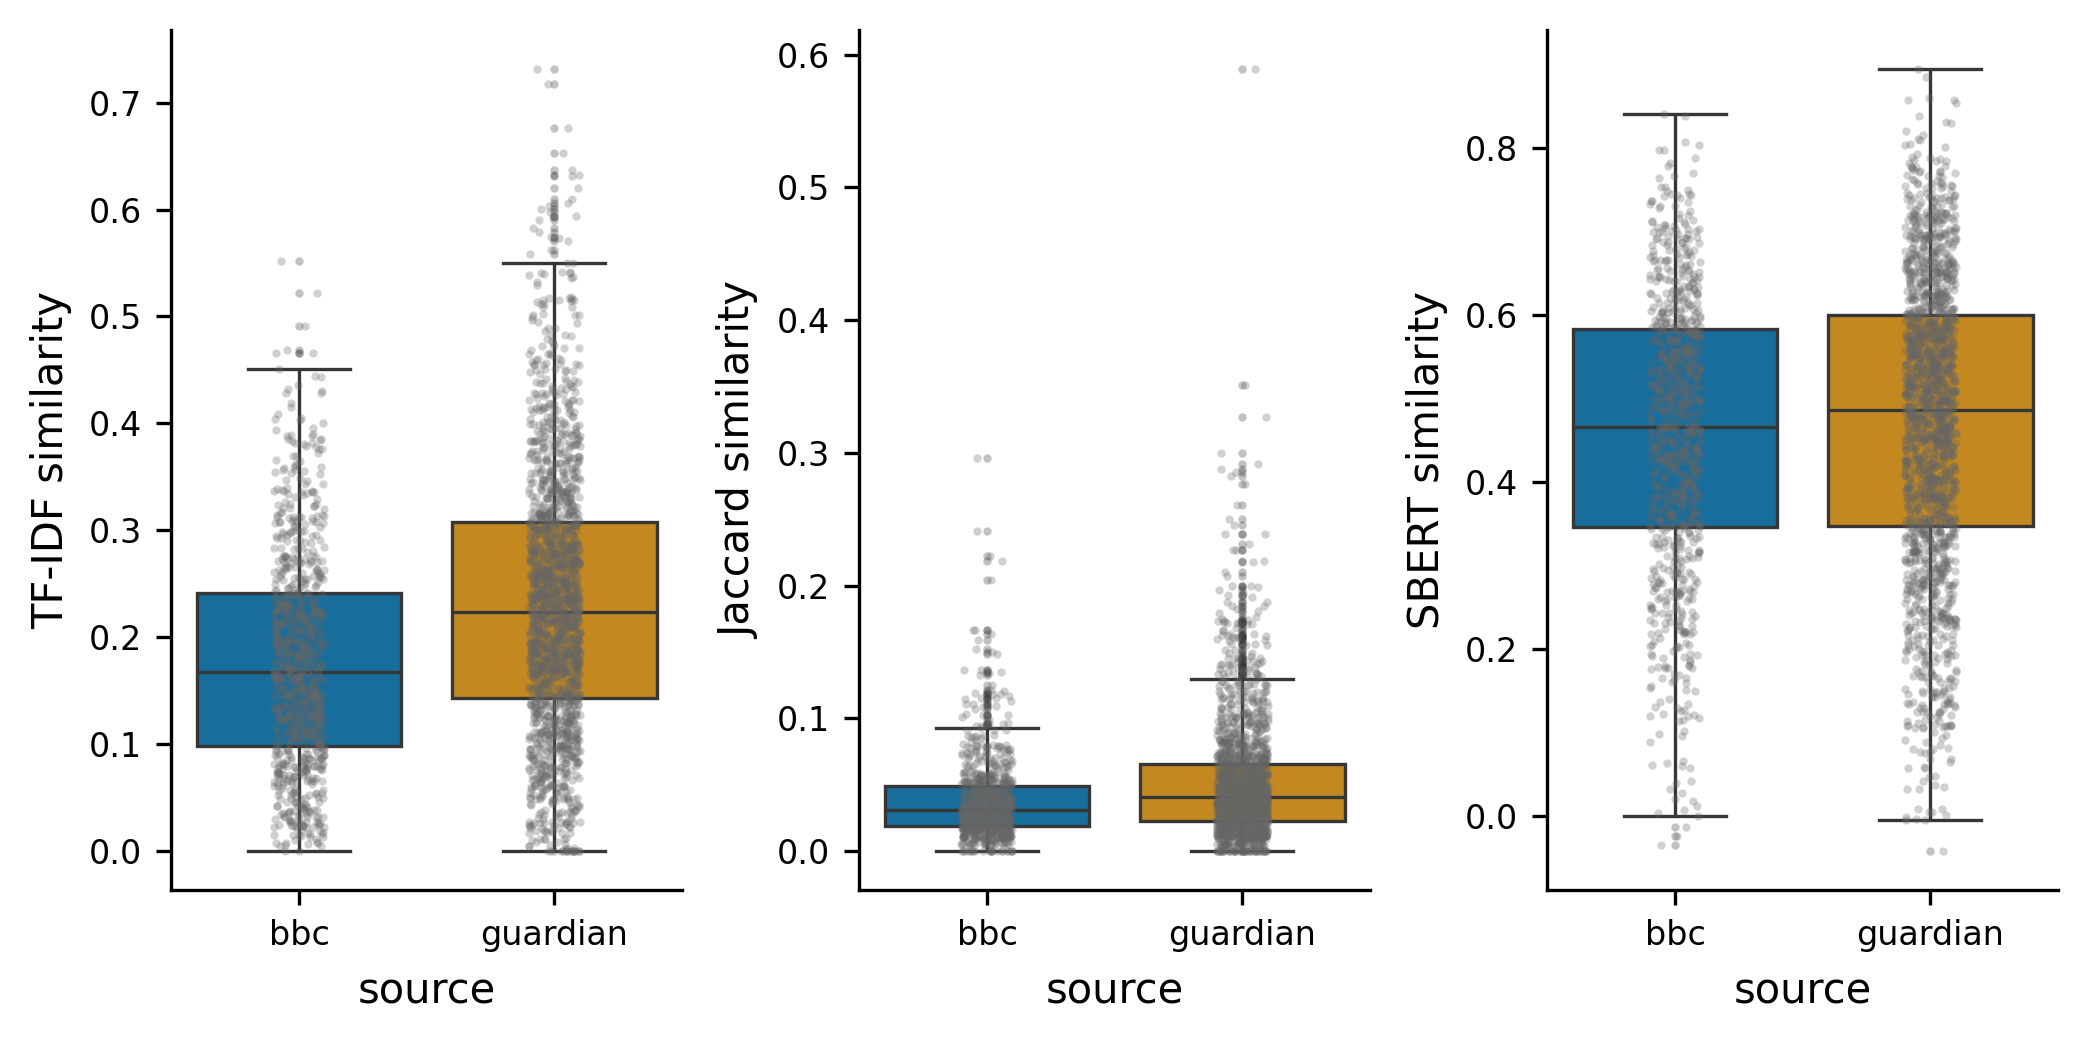
\includegraphics[width=\linewidth]{rq5_similarity_by_source.png}
  \caption{Similarity distributions by news source.}
  \label{fig:rq5_sim}
\end{figure}

\begin{figure}[h]
  \centering
  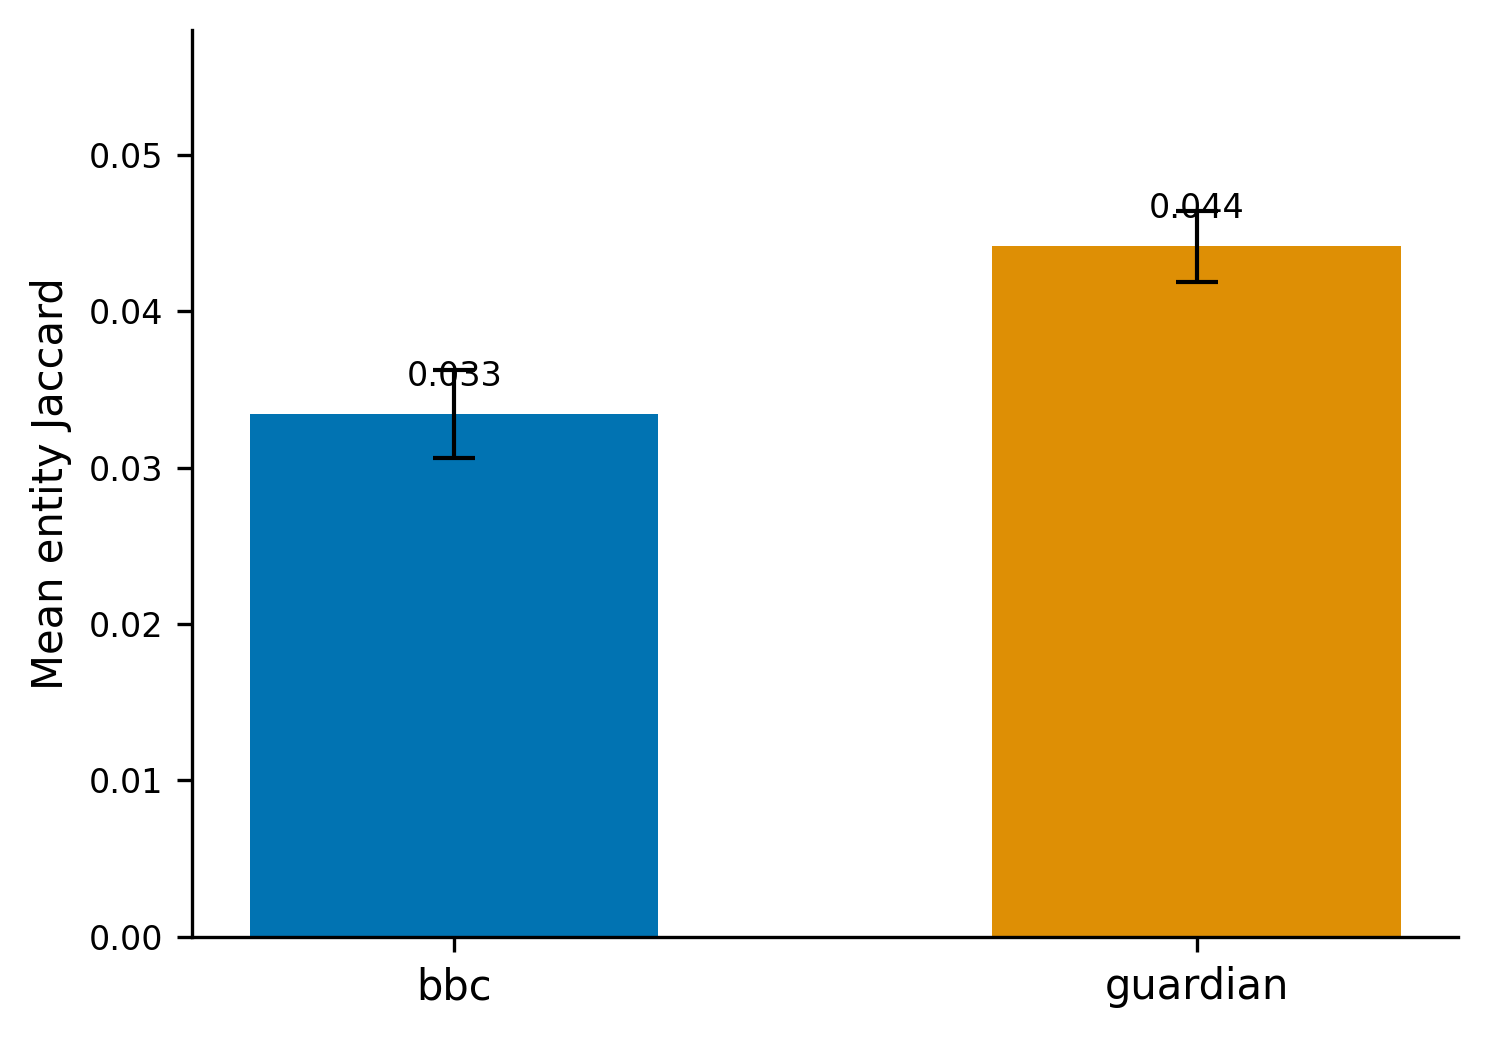
\includegraphics[width=0.85\linewidth]{rq5_entity_jaccard_by_source.png}
  \caption{Mean entity Jaccard per source (error bars: 95\% CI).}
  \label{fig:rq5_ent}
\end{figure}

\begin{table}[h]
  \centering
  \caption{Mean $\pm$ SD similarity by source; Kruskal-Wallis result.}
  \label{tab:rq5}
  \adjustbox{max width=\linewidth}{%
    \begin{tabular}{llll}
\toprule
source & TF-IDF & Jaccard & SBERT \\
\midrule
bbc & 0.178 ± 0.103 & 0.039 ± 0.031 & 0.457 ± 0.170 \\
guardian & 0.232 ± 0.124 & 0.052 ± 0.046 & 0.470 ± 0.175 \\
Kruskal-Wallis & H=111.62, p=0.000 & H=56.04, p=0.000 & H=3.18, p=0.075 \\
\bottomrule
\end{tabular}
%
  }
\end{table}

\begin{table}[h]
  \centering
  \caption{Dunn post-hoc pairwise $p$-values for SBERT similarity by source
           (Bonferroni corrected).}
  \label{tab:rq5_dunn}
  \adjustbox{max width=\linewidth}{%
    \begin{tabular}{lll}
\toprule
 & bbc & guardian \\
\midrule
bbc & 1.000 & 0.075 \\
guardian & 0.075 & 1.000 \\
\bottomrule
\end{tabular}
%
  }
\end{table}

% ============================================================
\section{Discussion}
\label{sec:discussion}

[Summarise and interpret findings across all five RQs. Discuss
implications for caption generation, news credibility, and multimodal NLP.
Acknowledge limitations: sample size, placeholder caption classifier, and
the use of article leads rather than full articles.]

% ============================================================
\section{Conclusion}
\label{sec:conclusion}

We have presented a multi-dimensional analysis of caption–article textual
similarity in news media, combining structural linguistic features, three
complementary similarity metrics, and named-entity alignment on a sample from
the VisualNews dataset. Our analysis reveals \ldots\ [fill in once results
are complete]. Future work includes implementing a supervised caption
type classifier (H2), scaling to the full VisualNews corpus, and extending
to non-English outlets.

% ============================================================
\bibliographystyle{plainnat}
\bibliography{references}

\end{document}